\documentclass{sig-alt-release2}

\usepackage{amssymb}
\setcounter{tocdepth}{3}
\usepackage{graphicx}
\usepackage{url}
\usepackage{subfigure}

%%%%%%%%%%%Añadido de CPB para controlar las versiones%%%%%%%
%Macros par los cambios
\usepackage[usenames]{color}
%\usepackage[dvips]{color}
\usepackage{colordvi}
\usepackage{ulem}
\normalem
\definecolor{MyDarkGreen}{rgb}{0,0.8,0.0}
\definecolor{MyDarkBlue}{rgb}{0,0,0.8}
\definecolor{MyDarkRed}{rgb}{0.6,0,0.0}
\newcommand{\borrar}[1]{\textcolor{MyDarkRed}{\sout{#1}}} %\sout}
\newcommand{\nuevo}[1]{\textcolor{MyDarkBlue}{\uline{#1}}} %\sout}
\newcommand{\nota}[1]{\textcolor{MyDarkGreen}{#1}} %\sout}
%%%%%%%%%%%%%%%%%%%%%%%%%%%%%%%%%%%%%%%%%%%%%%%%%%%%%%%%%%%%%%%%

\urldef{\mailsa}\path|cicamargoba@unal.edu.co|
\urldef{\mailsb}\path|cesarpedraza@usantotomas.edu.co|
% \newcommand{\keywords}[1]{\par\addvspace\baselineskip
% \noindent\keywordname\enspace\ignorespaces#1}

\begin{document}

\conferenceinfo{GECCO'11,} {July 12--16, 2011, Dublin, Ireland.} 
\CopyrightYear{2011} 
\crdata{978-1-4503-0690-4/11/07} 
\clubpenalty=10000 
\widowpenalty = 10000


% first the title is needed
\title{Intrinsic Evolvable Hardware for Combinatorial Synthesis Based on SoC+FPGA and GPU Platforms}

\numberofauthors{4}

\author{
\alignauthor
Carlos Camargo Bare�o\\
       \affaddr{Universidad Nacional de Colombia}\\
       \affaddr{Bogot�, Colombia}\\
       \email{cicamargoba@unal.edu.co}
\alignauthor
Cesar Pedraza Bonilla\\
       \affaddr{Universidad Santo Tom�s de Aquino}\\
       \affaddr{Bogot�, Colombia}\\
       \email{cesarpedraza@usantotomas.edu.co}
\and
\alignauthor
Luis Fernando Ni�o \\
       \affaddr{Universidad Nacional de Colombia}\\
       \affaddr{Bogot�, Colombia}\\
       \email{lfninov@unal.edu.co }
\alignauthor
Jose Martinez Torre\\
       \affaddr{Universidad Rey Juan Carlos}\\
       \affaddr{Madrid, Espa�a}\\
       \email{joseignacio.martinez@urjc.es}
}

%\authorrunning{Short form of author list} % if too long for running head


% the affiliations are given next; don't give your e-mail address
% unless you accept that it will be published
% \institute{Universidad Nacional de Colombia. \\  Facultad de Ingenier\'ia, Bogot\'a Colombia \\
% Universidad Santo Tom\'as \\  Facultad de Ingenier\'a de Telecomunicaciones, Bogot\'a Colombia \\
% \mailsa, \mailsb\\
% }

\maketitle

\begin{abstract}
Evolutionary algorithms are another option for combinatorial synthesis because they allow for the generation of hardware structures that cannot be obtained with other techniques. This paper presents a novel a parallel genetic programming (PGP) boolean synthesis implementation on a low cost cluster of an embedded platform called SIE, based on a 32-bit processor and a Spartan-3 FPGA. Some tasks of the PGP have been accelerated through a hardware coprocessor called FCU, that allows to evaluate individuals onchip as intrinsic evolution. Results have been compared with GPU and HPC implementations, resulting in speedup values up to approximately 2 and 180 respectively.  
\end{abstract}



% A category with the (minimum) three required fields
\category{B.5.2}{Hardware}{Register-transfer-level implementation}[optimization]

\terms{Design, Performance}

\keywords{Hardware copyleft, Embedded systems, Evolutionary algorithms, boolean synthesis, cluster}




\section{Introduction.}

One of the main goals in combinatorial synthesis consists of finding compact boolean expressions in the sum of products (SOP) form with the smallest possible number of variables and terms. Boolean algebra offers a way to find compact expressions, but this process depends on the designer's experience, resulting in non-optimal or inadequate expressions. There are other techniques available for combinatorial synthesis such as the Karnaugh maps, the Quine-McCluskey algorithm, the Reed-Muller algorithm. In general terms, these algorithms have disadvantages such as exponential complexity, lack of restrictions management, and multiple solutions. 

As an alternative to the traditional design of combinatorial circuits, some authors have proposed bio-inspired techniques to create combinatorial circuits that can not be obtained with the traditional methods and to add some restrictions to the design such as delay, area, etc. Nicholson \cite{Nicholson} has used Simple Genetic Algorithms (SGAs) with a fixed length representation for small problems, Kajitani \cite{Kajitani:1996p16} has worked with Variable-length Genetic Algorithms (VGAs) evolving up to 6-bit problems. Aguirre \textit{et al} \cite{Aguirre:2009p66} used tree-based genetic programming (GP) for evolving small circuits, Xu \cite{Xu2009} has worked with adaptive immune GA obtaining only 4-variable circuits, as well as Coello with ant colony algorithms \cite{coello2000}. Others authors have proposed a platforms to use reconfiguration techniques with hard-time restrictions due the high reconfiguration latency \cite{UpeguiS06,MorenoTS05,UpeguiS05}. 

One of the main problems to create circuits by using these techniques is the response time, due the high computational requirements for implementing any bio-inspired algorithm. As a result, only small circuits can be created in reasonable time \cite{Vasicek2008, koza2005}.
To solve the scalability restriction of creating digital circuits by using parallel genetic programming (PGP), we have developed a low cost cluster-based SoC + FPGA  architecture called SIE. A fitness coprocessor unit (FCU) was developed on each FPGA in order to accelerate the convergence of a Intrinsic PGP (individuals are tested in the same platform), as well as provides an appropriate support for 8 variables synthesis problems. 


These strategies allow to create combinatorial blocks that cannot be obtained with traditional methods, and to add some restrictions to the design such as delay and area. These designs have a very low limited number of variables \cite{DGJH98} and they are mainly oriented to obtain a few basic structures.

In order to use parallel genetic programming (PGP), an FPGA cluster-based architecture to solve the combinatorial synthesis problem on-chip has been developed. The fitness coprocessor unit (FCU) on each FPGA helps to accelerate the convergence of the algorithm, as well as provide an appropriate support for 12-variable synthesis problems. The success of the system is mainly due to the capability of evaluating a chromosome in the FPGA through a virtual LUT-oriented architecture without using high-latency partial reconfiguration techniques, and determining the fitness value for an individual faster than other related works. 

Due to that the capability of GP to run on massive parallel architectures, the proposed synthesis algorithm was compared to a High Performance Cluster (HPC) and a graphics processing unit (GPU) implementations. 

% &&&&&&&&&&&&&&&&&&&&&&&&&&&&&&&&&&&&&&&&&&&&&&&&&&&&&&&&&&&&&&&&&&&&&&&&&&&&&&&&&&&&&&&&&&&&&&&&&&&&
%                                                                     PROGRAMACION GENETICA 
% &&&&&&&&&&&&&&&&&&&&&&&&&&&&&&&&&&&&&&&&&&&&&&&&&&&&&&&&&&&&&&&&&&&&&&&&&&&&&&&&&&&&&&&&&&&&&&&&&&&&
\section{Genetic Programming in combinatorial Synthesis}
This section describes some of the most important aspects of the proposed evolutionary algorithm for the combinatorial synthesis problem, such as chromosome representation, the fitness problem and the genetic operators.

\subsection{Chromosome representation.}
The codification is the way a logic circuit is represented using a bit array in order to be used in the evolution process \cite{FR06}. This representation must be able to represent all the different solutions to the problem, also the crossover and mutation operators should not generate infeasuble individuals, and it must cover all the solution space. There are different ways of representing combinatorial hardware for a genetic algorithm: tree-based representation in 2-D, PLD-like structures and cartesian representation are some of them \cite{JKFB+99} \cite{THTN+92} \cite{JMPT98}.

The 2-D tree representation is appropriate for implementing parallel systems because it allows splitting the chromosomes for balancing the computational load \cite{QYCC06}. Figure \ref{fig:cell_structure} shows the selected cell-based structure representation. Each basic cell has 3 functions $f$ and 4 input variables $v$ coded in binary. This representation allows the addition of more cells to represent larger circuits. It must be mentioned that the chromosome length has to be variable because the length of the solution to the synthesis problem is unknown a priori. 

\subsection{Fitness function.}
Finding the appropriate fitness function is important because it is responsible for quantifying the way a chromosome or individual meets or does not meet the requirements.


\begin{figure}[htpb]
\begin{center} 
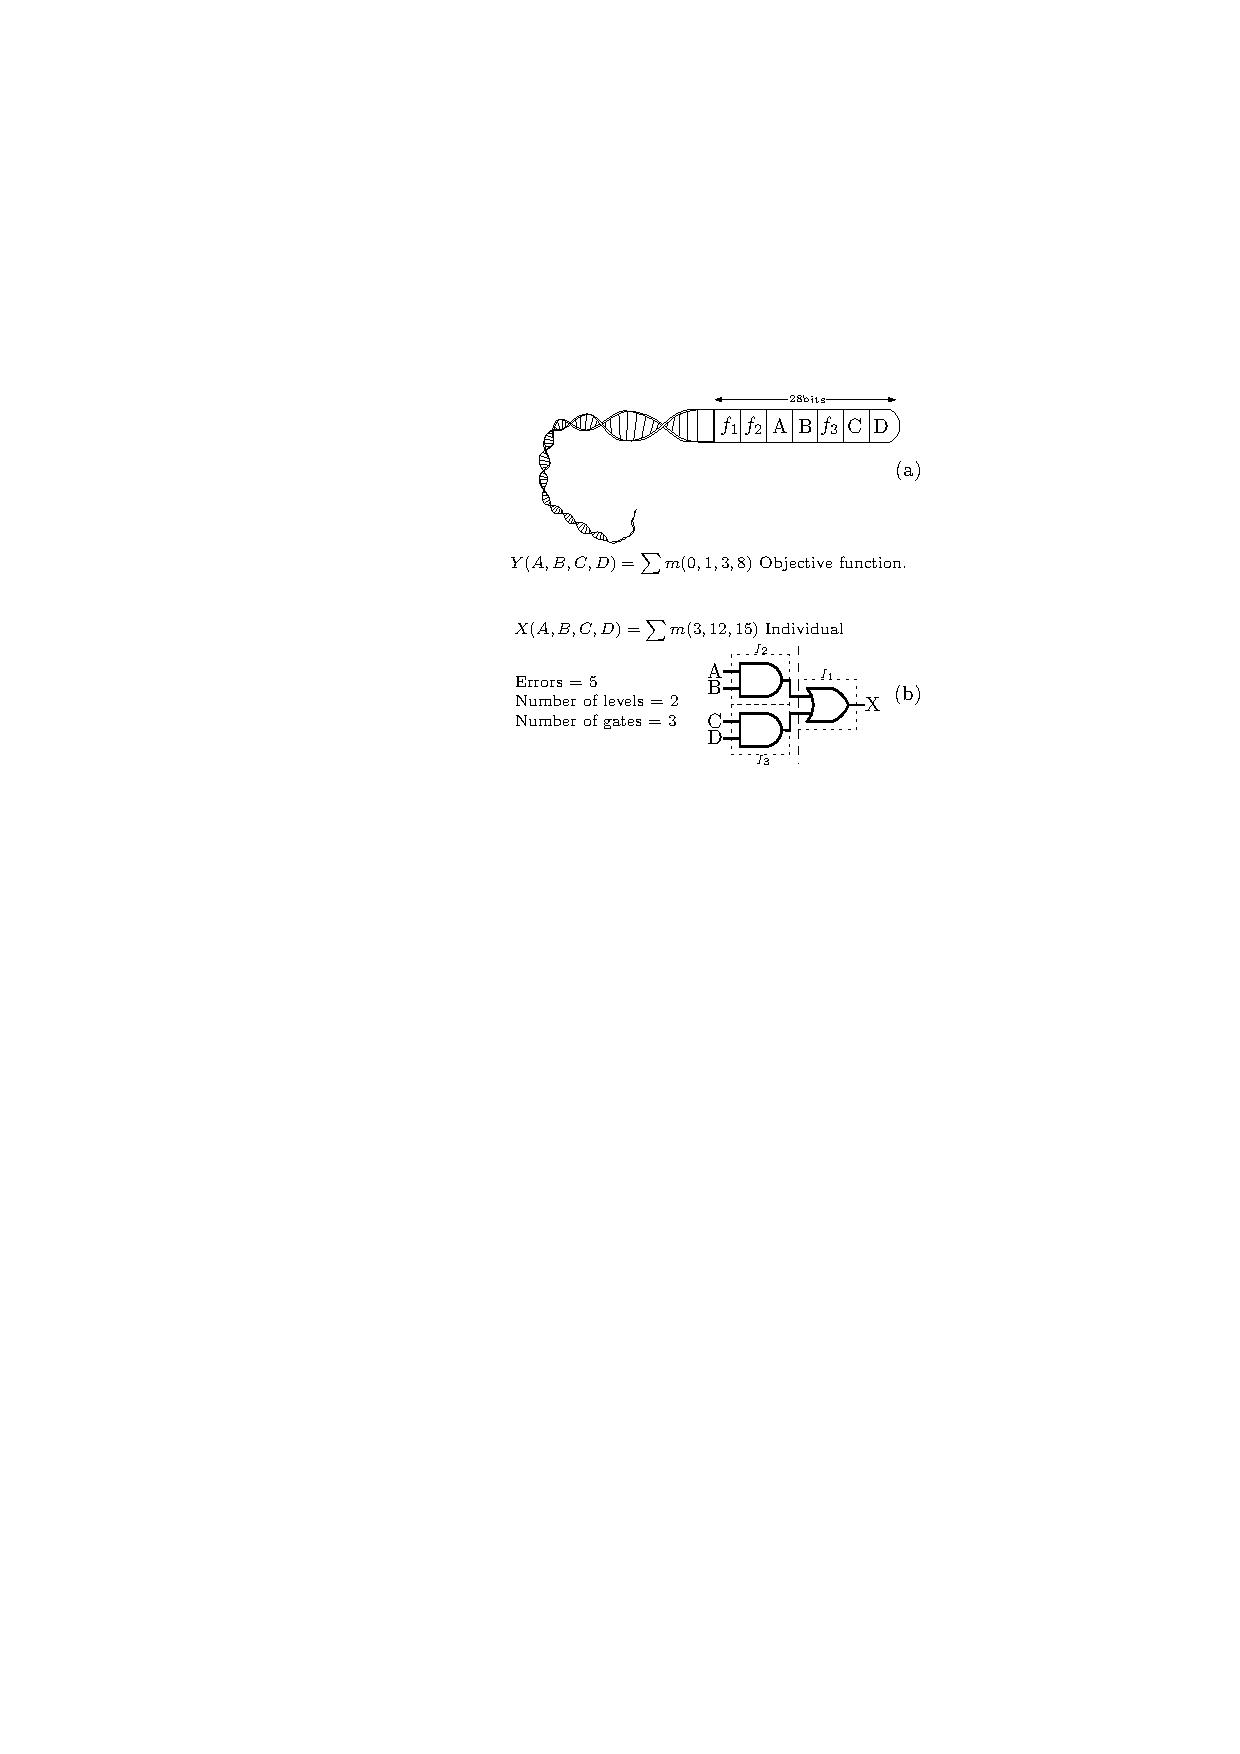
\includegraphics[width=7cm]{./images/fitness} \end{center}
\caption{Cell-based structure representation.}\label{fig:cell_structure}
\end{figure}


\begin{equation}
\label{fitness}
fitness=\omega_{1} . [ \sum_{j=1}^m \sum_{i=1}^n Y(j,i)-X(j,i) ] + \omega_{2}.P(x) + \omega_{3}.L(x)
\end{equation}


In equation \ref{fitness} the fitness function for the proposed GP is shown. Constants $\omega_{1}$, $\omega_{2}$ and $\omega_{3}$ are used for establishing the weights of each of the parameters that will determine the fitness function. The double-summation term calculates the number of matches of the individual X for all the possible combinations at the output with the target functions Y; the $P(X)$ function is used for calculating the number of logic gates of a chromosome taking into account some of the $introns$ or segments of the genotype string that will not have any associated function and that do not contribute to the result of the logic circuit that they represent. The function $L(X)$ is used for determining the number of levels the circuit has, or in other words the number of gates that the critical path crosses. The $m$ constant is the number of outputs in the circuit and $n$ the number of possible combinations of inputs in the circuit.

\subsection{Genetic operators.}
The selection operator is responsible for identifying the best individuals of the population taking into account the exploitation and the exploration \cite{QYCC06}. The first one allows the individuals with better fitness to survive and reproduce more often, and the second one means searching in more areas and making it possible to find better results. In the other hand, the mutation operator modifies the chromosome randomly in order to increase the search space. It can change: 1) an operator or variable and 2) a segment in the chromosome. Both are executed randomly with a certain probability. A variable mutating probability during the execution of the algorithm (evolvable mutation) \cite{RKYZ02} is more effective for evolvable systems. Finally, the crossover operator combines two selected individuals for obtaining two additional individuals to add to the population. A crossover system with one or two crossover points randomly selected has been implemented because it is more efficient for evolvable systems \cite{JMPT98b}.


% &&&&&&&&&&&&&&&&&&&&&&&&&&&&&&&&&&&&&&&&&&&&&&&&&&&&&&&&&&&&&&&&&&&&&&&&&&&&&&&&&&&&&&&&&&&&&&&&&&&&
%                                                                     PROGRAMACION GENETICA 
% &&&&&&&&&&&&&&&&&&&&&&&&&&&&&&&&&&&&&&&&&&&&&&&&&&&&&&&&&&&&&&&&&&&&&&&&&&&&&&&&&&&&&&&&&&&&&&&&&&&&

\section{Copyleft SIE platform.}
The hardware project copyleft SIE \cite{CC11b} \cite{CC11d} created by our team work, is composed of a custom embeddded platform and a software development kit based on Linux operating system; allowing the generation of commercial applications under the Creative Commons BY-SA licenses, which allows the distribution and modificacion of the design (including commercial applications), with only the requirements that the derived products be under the same license and that the proper credit be given to the author of the original work. This is what defines the base of the \textit{hardware copyleft} products.

\subsection{The SIE Platform.}

The SIE platform is composed by a System-On-a-Chip processor and a FPGA (Figure \ref{SIE_arch}). The SoC is a MIPS processor (Ingenic JZ4725) running at 400MHz with peripherals that allows to control: a 2GB NAND memory for file storage, a 32MB SDRAM, a serial communication channel (UART), micro-SD memories, I2C port, 3-inch color LCD display, 2 input and 1 output audio stereo interfaces and 2 analog inputs. The XC3S500E Xilinx FPGA gives 25 GPIOs and controls an 8 channel analog-to-digital converter. There are two communication channels between the FPGA and the processor, the first one is a JTAG that allows the FPGA configuration and the execution of tests to the implemented circuits. The data, address and control buses are part of the second channel, which is used to exchange information between the processor and the peripherals implemented inside the FPGA.

\begin{figure}[htpb]
   \begin{center} 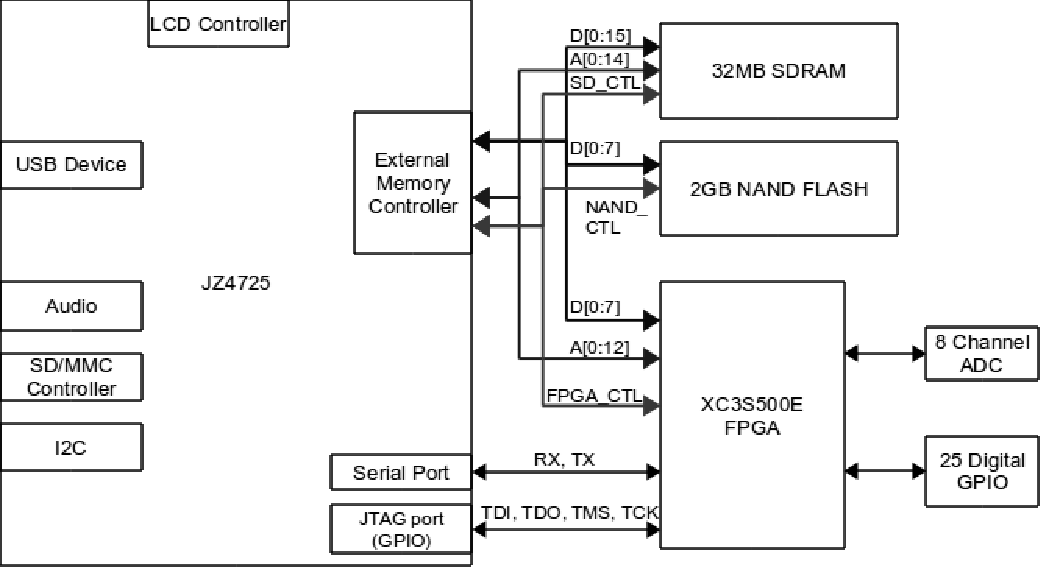
\includegraphics[scale=.45]{./images/SIE_block_diagram.pdf}   \end{center}
    \caption{SIE development platform structure} \label{SIE_arch}
\end{figure}

SIE provides power connection through a USB port, which is also configured as a network interface. This allows the file transfer and the execution of a remote console using the \textit{ssh} protocol. This communication channel can also be used to configure the non-volatile NAND memory, which simplifies the whole configuration of the platform through the USB port.


SIE provides an economical alternative (70 USD per node) for implementing evolutionary algorithms; Vasicek et al. \cite{RORA+07}, Higuchi et al. \cite{JJPR} and Sekanina\cite{ZVLS07} use architectures based on Xilinx Virtex 2 Pro family for implementing similar applications, closed to 1000 USD y 3000 USD per node.  By separating the FPGA and the processor and providing a communication channel between them, SIE can use cheaper devices (4 USD for the processor, 10 USD for the FPGA) reducing significantly the cluster's costs. On the other hand, selected GPU for the present work is about 200 USD.


\section{GP Implementation} 
The GP was implemented in two stages: the first one is about software development and its parallelization on HPC and GPUs, and the second one refers to a hardware implementation to speed it up on the SIE plataform.

\subsection{Parallel software design.}
\subsubsection{HPC}
Natural evolution works with a whole population not with a single individual (except for selection and reproduction) some operations can be done separately, therefore almost all operations in a GP are implicitly parallel. Using the island approach, the population is divided into sub-populations that will evolve in each processor of the cluster or parallel architecture. Figure \ref{fig:communications} shows the GP communications scheme in the parallel system. When the system starts, each processor receives the objective function (i.e, a true table), creates its sub-population and starts the evolution process, consisting of fitness evaluation, selection, crossover, mutation and reproduction. Once the system reaches a number of generations, some individuals are selected to be transfered from one processor to another one. A master processor is in charge of collecting the in-transfer individuals and moving them to the rest of the nodes (slaves), 

Increasing the probability of convergence of the algorithm \cite{cantu:2001}. The ratio of data exchange (the number of the best individuals to exchange increases the probability of finding a better solution) and migration frequency are important parameters to improve the performance of the algorithm. 

To implement communications in SIE, a custom message passing library was created to program the distributed system. Standard libraries such Open MPI  executes on SIE with a very low performance, due they were designed for robust platforms.

\begin{figure}[htpb]
\begin{center} 
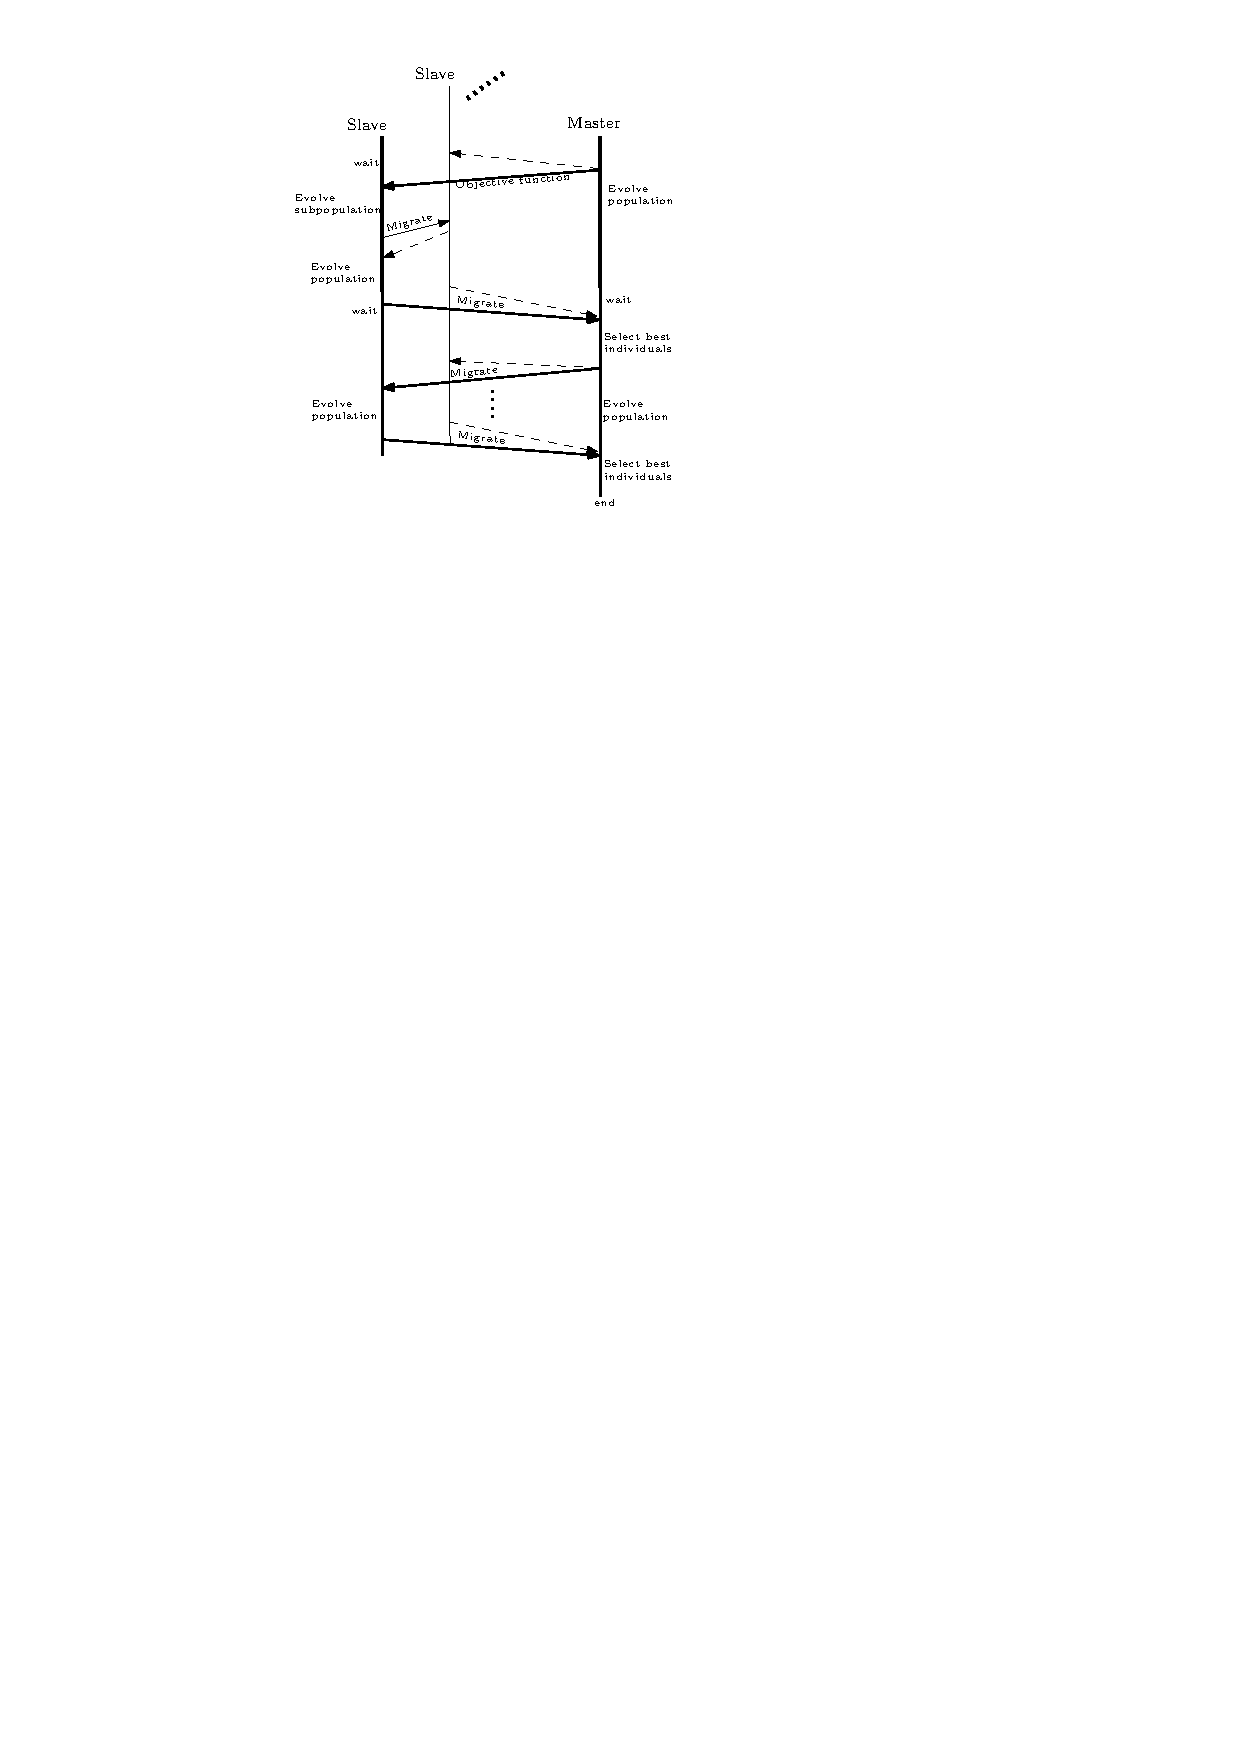
\includegraphics[width=6cm]{./images/communications} \end{center}
\caption{GP communications scheme in parallel architecture.}\label{fig:communications}
\end{figure}


\subsubsection{GPU.}
Two main parts can be identified to implement the system on GPUs. The first part involves the random number generation and the second one the GP as such. The GP requires random numbers for generating an initial population and then to mutate and cross their individuals. Due that a GPU can not generate random numbers by using C classical libraries, it is necessary generate them in a different way. Generate these numbers on CPU and then transport them to the GPU is not viable because it takes a lot of system clocks. To solve this problem a Mersenne-twister algorithm is executed on the GPU before the $kernel-GP$ to make a buffer of random numbers on its own global memory.


\paragraph{Kernel structure.}
Figure \ref{fig:migration_scheme} shows the way the GP has been implemented on the graphics device. A thread $t$ executes a $kernel-GP$ (a common segment of code that process different data in each instance), and generates a $\mu$-population, performs the operators of selection, mutation and crossover a number of generations required. After $P$ generations, $M$ individuals will be transferred to the global memory and then to the host device (CPU system). $P$ is known as the frequency of migration and the $M$ number is called the migration factor.

\begin{figure}[htpb]
\begin{center} 
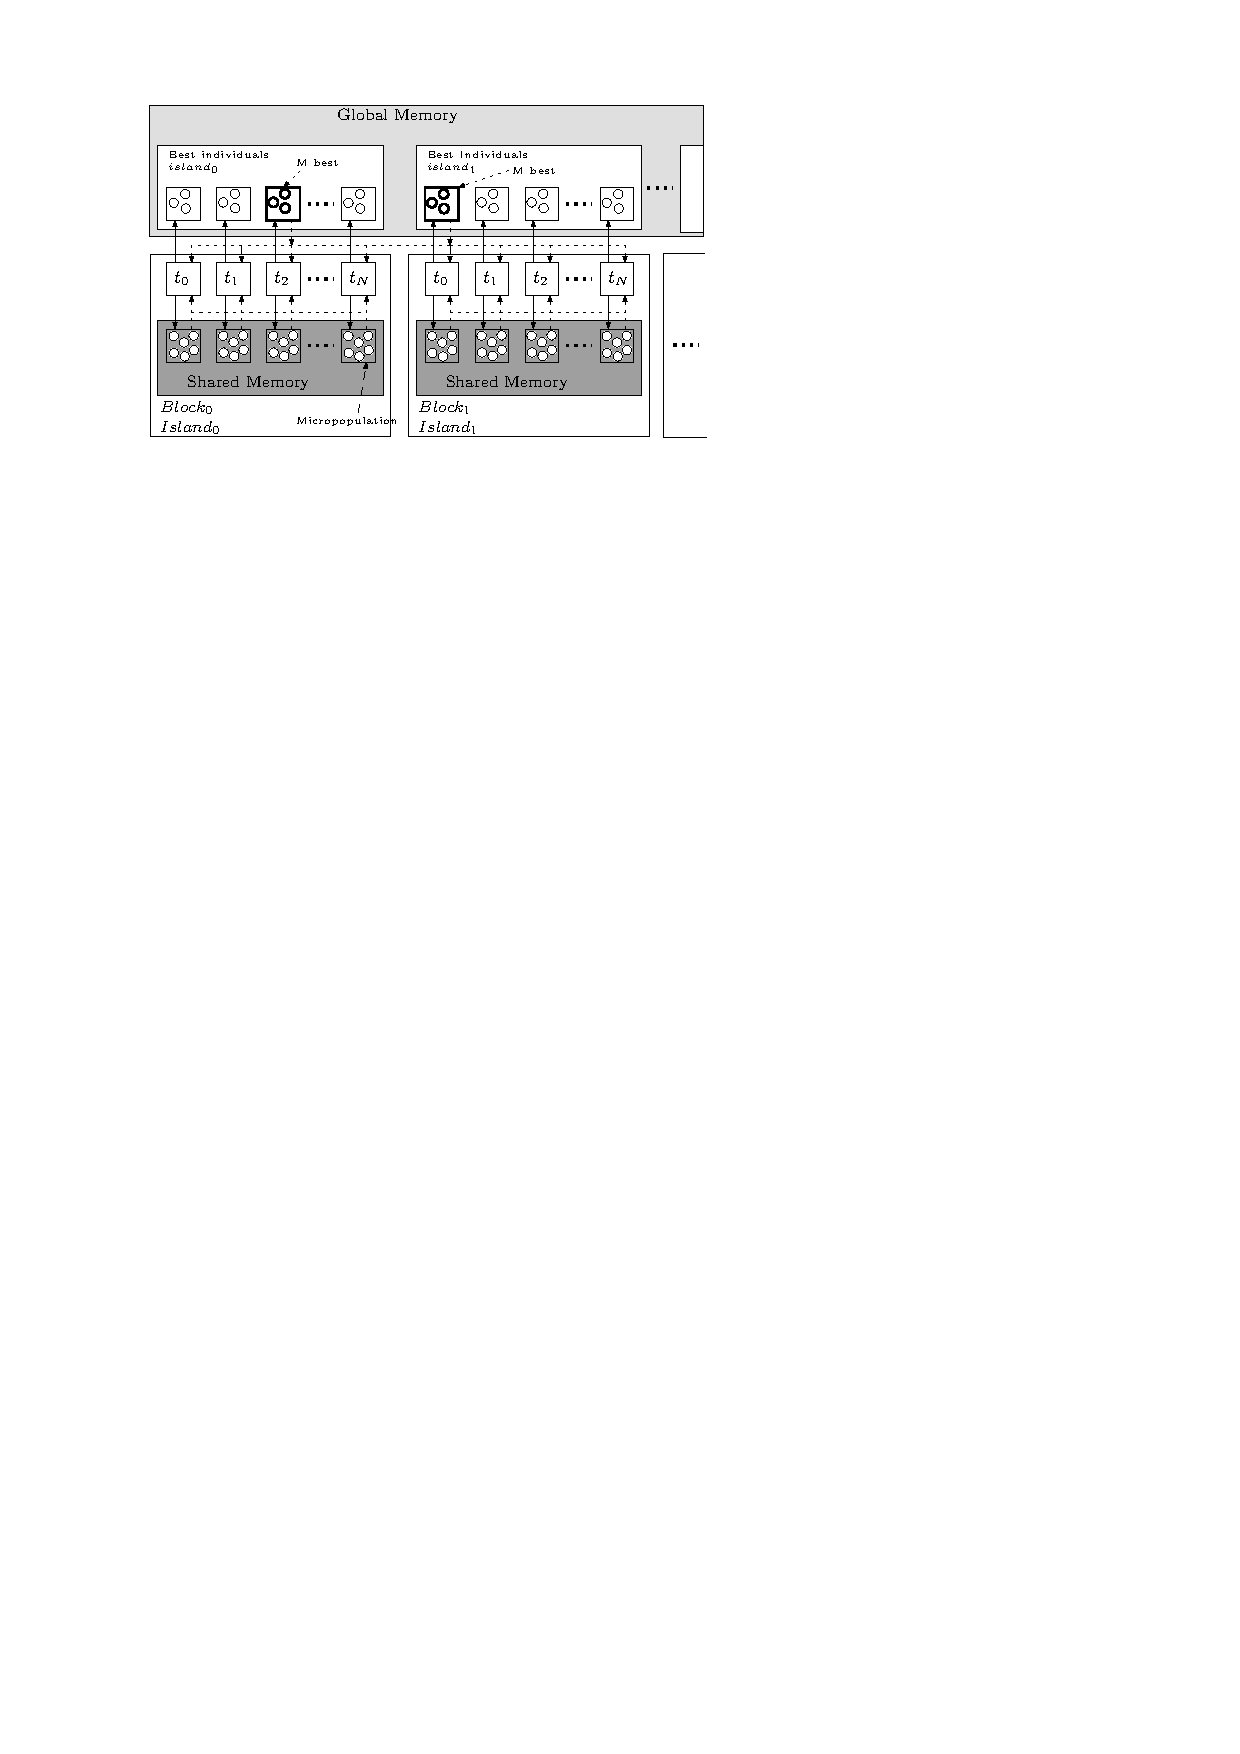
\includegraphics[width=8cm]{./images/migration_scheme} \end{center}
\caption{GPU implementation of the evolvable algorithm.}\label{fig:migration_scheme}
\end{figure}

Also, it can be observed that each thread can cooperate with other threads inside the same block through shared memory, sharing the best individuals and improving the efficiency of the GP.



\subsection{Hardware design.}
In the second stage a profiling of the software implementation with gprof tool, determined that the most costs were the fitness function calculation and the new individual generation (25\% and 35\% of the execution time, respectively).

Therefore, these two steps have been accelerated with a dedicated hardware in the FPGA. The Fitness Calculation Unit (FCU, see Figure \ref{fig:hw_block}) is the hardware element designed in order to accelerate this processes. This coprocessor is connected to the JZ4725 processor through its custom interface (using data, address, control buses).  

Inside the FCU, the chromosome passes from the DRAM memory to local memory through the custom interface, and each of its basic cells are converted to an equivalent Virtual Look Up Table (VLUT) with a ROM based translation. Then the number of wrong minterms is calculated using the information from the objective function and a counter as input. Finally, the FCU calculates the final fitness value including the number of gates and the critical path, and will be sent back to the JZ4725 processor. In order to speed up pseudo random number generation, a Mersenne-Twister-based coprocessor was inserted through the same custom interface. 

\begin{figure}[htpb]
\begin{center} 
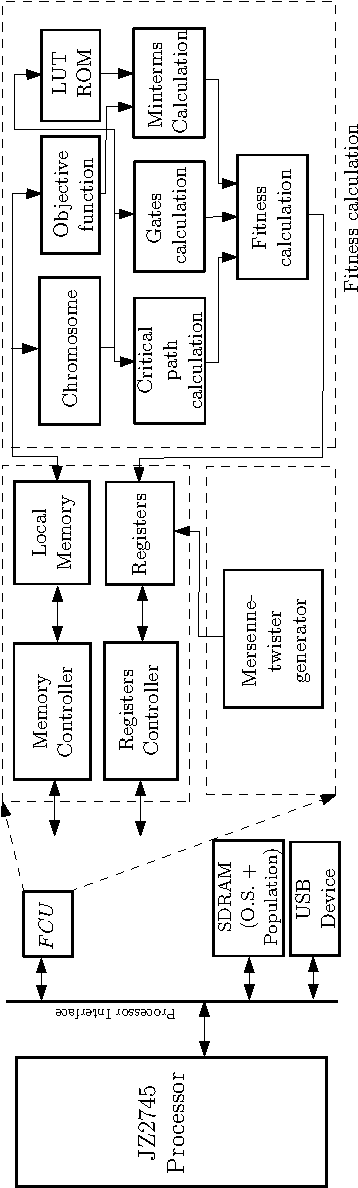
\includegraphics[width=8cm]{./images/hw_block_diagram} \end{center}
\caption{FCU structure.}\label{fig:hw_block}
\end{figure}



% &&&&&&&&&&&&&&&&&&&&&&&&&&&&&&&&&&&&&&&&&&&&&&&&&&&&&&&&&&&&&&&&&&&&&&&&&&&&&&&&&&&&&&&&&&&&&&&&&&&&
%                                                      EVALUACION
% &&&&&&&&&&&&&&&&&&&&&&&&&&&&&&&&&&&&&&&&&&&&&&&&&&&&&&&&&&&&&&&&&&&&&&&&&&&&&&&&&&&&&&&&&&&&&&&&&&&&
\section{Performance evaluation.}

To obtain the performance and prove the scalability of the algorithm in SIE, it was compared to two parallel architectures. The first one is a High Performance Computer (HPC) called ALTAMIRA. The HPC setup is made up of 18 eServer BladeCenters with 256 JS20 nodes (512 processors), using a Myrinet network with 1 Gbps bandwidth. The second platform is a GPU architecture based on a NVIDIA GTS450, made by 192 CUDA cores, each one working at 1,56 GHz and a DDR5-1GB global memory.

On the other hand, the SIE configuration is made up of 6 JZ4725-FPGA nodes with the architecture described above. The response time is measured for the parallelized versions of the GP in both ALTAMIRA and SIE. Several scenarios have been tested with different input parameter configurations: 1) number of input variables (4, 8 or 12, corresponding to a comparator problem of 2, 4 and 6 bits); 2) population size (512, 1024 or 2048) and 3) number of nodes running the experiment, ranged from 1 to 6 in SIE, and 2 to 16 or 64 in ALTAMIRA. The first and second parameters determine the size of the problem. The last one gives an idea about the scalability of the system.



\subsection{Response Time.}
Figure \ref{fig:rt_vars} shows the response time for both platforms with different numbers of nodes and variables with 1024 individuals during 100 generations. These results show the high performance of SIE cluster for the algorithm. This experiment demonstrates that the response time for SIE does not depend on the size of the problem. In contrast, response time in ALTAMIRA has a high dependency of the size of the problem, because individuals had to be evaluated by software.


Figure \ref{fig:rt_indv} shows the response time in both architectures when varying the number of individuals of the population. It is observed that both architectures have a strong dependency of the number of individuals in the algorithm. This is because increasing this number causes an increment of the software computational load for both clusters. Even in this scenario, SIE shows an excellent performance compared to ALTAMIRA.

%NOTA DE NI�O: COMO LO OBSERVO??
%%%%%%%%%%%%%%%%%%%%%


\begin{figure}[h!]
\begin{center}
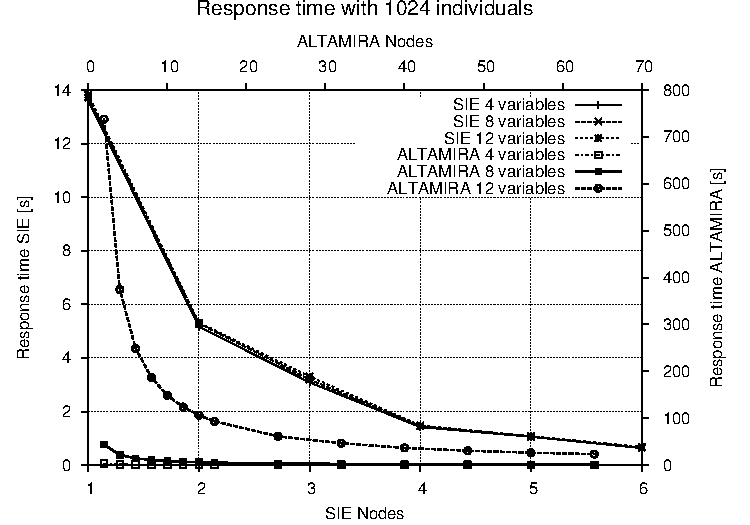
\includegraphics[width=8cm]{./images/response_time_1024indiv} 
\end{center}
\caption{Response time in SIE and ALTAMIRA for different number of variables.}
\label{fig:rt_vars}
\end{figure}

\begin{figure}[h!]
\begin{center} 
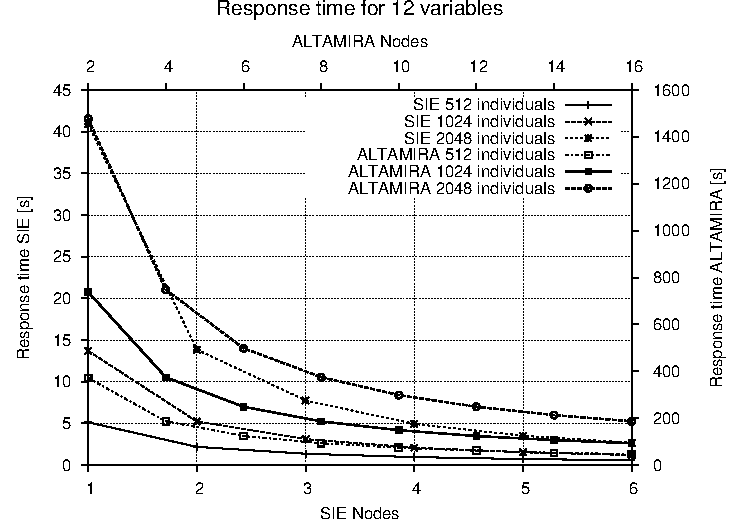
\includegraphics[width=8cm]{./images/response_time_12var} 
\end{center}
\caption{Response time in SIE and ALTAMIRA for different number of individuals.}
\label{fig:rt_indv}
\end{figure}
%%%%%%%%%%%%%%%%%%%%%

Figures \ref{fig:rt_gpu3d} shows the response time of executing the GP in the graphics hardware with problems of 4, 8 and 12 variables are fixed. Varying the number of islands and threads, can be observed that the best scenario is obtained when the number of threads is increased independently the number of islands. This is because when more threads are launched more parallelism is performed in the system, until the maximum of threads permitted by the GPUs is reached.


%NOTA DE NI�O: NO SE ENTIENDE PORQUE FALTA DEFINIR EL MARCO DE TRABAJO, COMO SE REALIZ� LA PRUEBA
%%%%%%%%%%%%%%%%%%%%%


\begin{figure}[h]
\begin{center} 
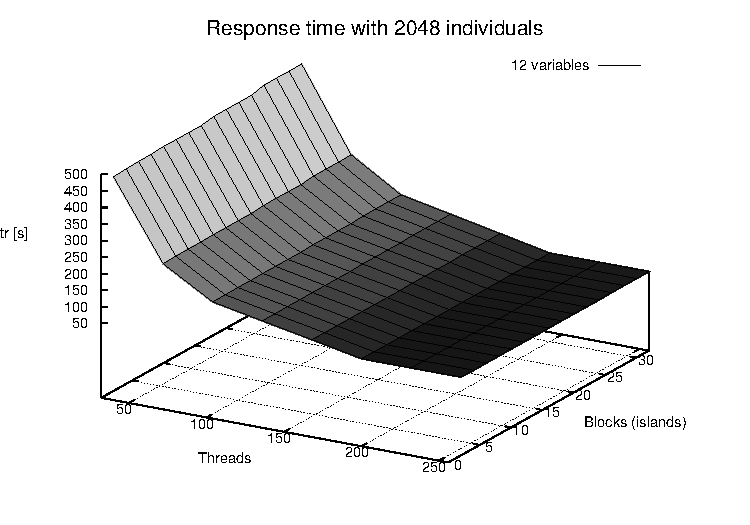
\includegraphics[width=8cm]{./images/response_time_threads_cuda_12var}
\end{center}
\caption{Response time of the algorithm in NVIDIA GTS450 GPU.}
\label{fig:rt_gpu3d}
\end{figure}


\begin{figure}[h!]
\begin{center} 
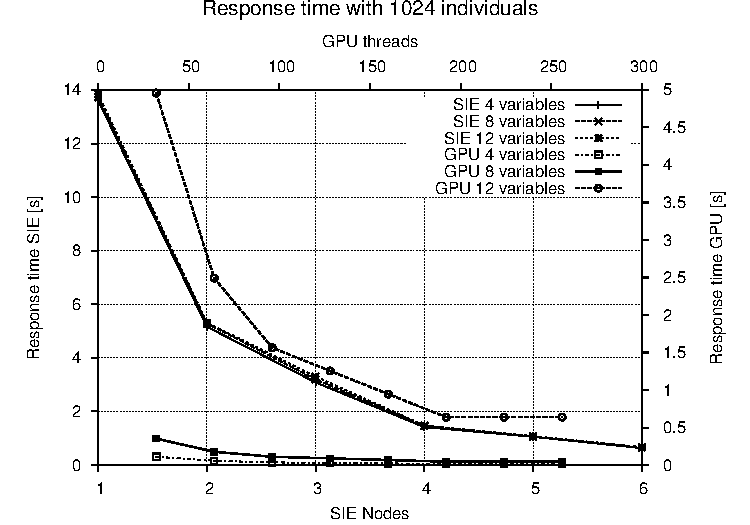
\includegraphics[width=8cm]{./images/response_time_1024indiv_gpu} 
\end{center}
\caption{Response time in SIE and GPU for different number of individuals.}
\label{fig:rt_indv2}
\end{figure}



\subsection{Speedup.}
The speedup of the SIE vs ALTAMIRA for different number of variables is presented in figure \ref{fig:speedup1} with the number of variables fixed to 12. The excellent performance of SIE can be explained because individuals have been directly tested in hardware (FPGA), obtaining a combination of their true table on each cycle of the system clock. On the other hand, individuals evaluated in software by ALTAMIRA require a lot of system clocks, causing response times hundreds of times higher than SIE.                                                     

%%%%%%%%%%%%%%%

%NOTA DE CAIN: Aca se debe hablar de la ventaja de utilizar la arquitectura propuesta basada en la LUT virtual y de como es conveniente implementarla en HW, ya que se demuestra que en SW va mas lento.

%%%%%%%%%%%%%%%


\begin{figure}[h!]
\begin{center} 
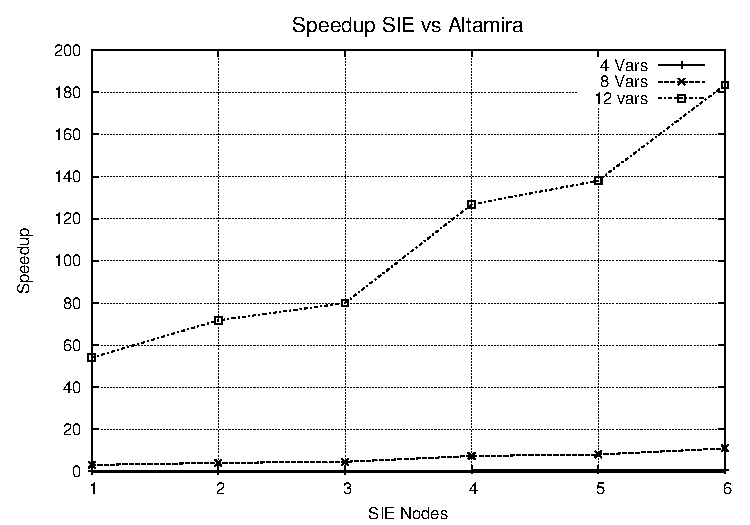
\includegraphics[width=8cm]{./images/speedup_sie_vs_altamira} 
\end{center}
\caption{Speedup of SIE vs Altamira comparing 1 SIE node = 2 Altamira nodes.}
\label{fig:speedup1}
\end{figure}

On the other hand, figure \ref{fig:speedup2} shows the speedup number when SIE and GPU are compared. It can be observed that SIE performance is higher than GPU only when 12-variables problems are evolved.  This can be explained because the whole population have been tested in hardware, obtaining a combination of their output on each cycle of the system clock. But, when an individual is tested in software, each combination requires a set of instructions, that requires a lot of cycles of the system clock.

The obtained speedup number is significant (about 50 and 180) when SIE is compared against ALTAMIRA. In \cite{SEKANINA2008, ABYSEK2010} the obtained speedup is about 30-40 when 1 accelerator processor was used and compared against a single PC.

\begin{figure}[h!]
\begin{center} 
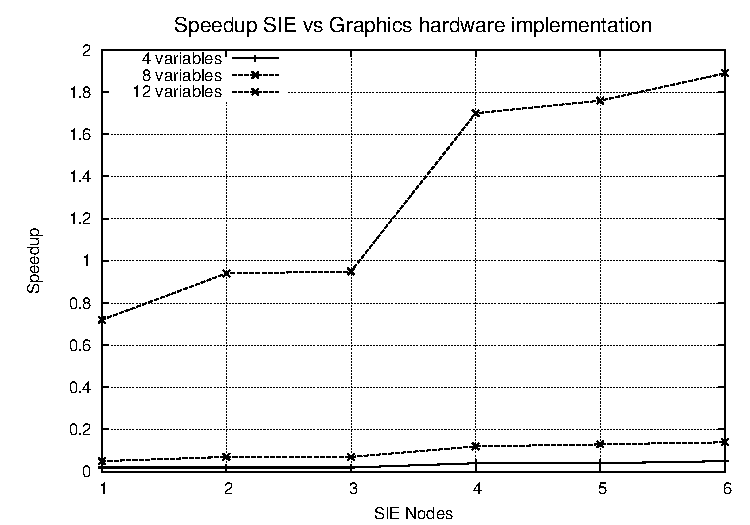
\includegraphics[width=8cm]{./images/speedup_sie_vs_cuda} 
\end{center}
\caption{Speedup of SIE vs GPU comparing 1 SIE node = 32 threads.}
\label{fig:speedup2}
\end{figure}



% &&&&&&&&&&&&&&&&&&&&&&&&&&&&&&&&&&&&&&&&&&&&&&&&&&&&&&&&&&&&&&&&&&&&&&&&&&&&&&&&&&&&&&&&&&&&&&&&&&&&
%                                                                     CONCLUSIONES Y TRABAJO FUTURO
% &&&&&&&&&&&&&&&&&&&&&&&&&&&&&&&&&&&&&&&&&&&&&&&&&&&&&&&&&&&&&&&&&&&&&&&&&&&&&&&&&&&&&&&&&&&&&&&&&&&&

\section{Conclusions and future work.}
This paper presented a novel way to evaluate individuals in an intrinsic evolvable algorithm on an open embedded platform called SIE, and results were compared to an HPC called ALTAMIRA and a high performance NVIDIA GPU. To accelerate the evolution process, a coprocessor was implemented to calculate the fitness function and to generate random numbers, improving the performance for problems with more than 6 bits. 

Results showed a speedup of 2 when SIE was compared to GPU, even when 192 processing cores were used in the last one. When compared with ALTAMIRA, SIE showed a speedup up to 180, due the high computational load in software when 16 nodes were used in ALTAMIRA. Significant speedup numbers were obtained due individuals have been directly tested in hardware, getting a combination of their true table on each cycle of the system clock. In the other hand, when an individual is tested in software, each combination requires a set of instructions, that requires a lot of cycles of the system clock.


Tests proved that the algorithm is more effective for 4-bit and 8-bit problems. 12-bit problems in SIE had excellent performance, but because the search space is too long, converging to a suitable solution was difficult for the algorithm. This problem could be solved as future work with some improvements in terms of multiple FCUs inside an FPGA, more nodes, and other hardware-accelerated genetic operators.



\bibliographystyle{plain}
\bibliography{./biblio_EHW.bib}

\end{document}
